Testing is an important part of any kind of development, be it software development or other kinds of development.
This section presents the different kinds of tests performed.

\section{Performance}

The reported maximum frequency of the synthesized processor with the default performance optimization settings is 133.500Mhz, i.e. a minimum clock period of 7.491ns.
Enabling the same optimization flags as in \cite{assignment-1}, and with the optimization effort set to high, the reported maximum frequency of the optimized processor is 137.578MHz.

\section{Energy Efficiency}
\label{results:energy-efficiency}

Xilinx ISE's integrated Xilinx Xpower Analyzer can generate power usage reports based on VHDL designs.
However, when generating power analysis reports, it unfortunately incorrectly assumed that the clock signals in the processor design had a clock frequency of 0 Mhz.
Because of this, the measurements are considered to be of low accuracy.
Still, this report is useful for getting a vendor-assisted power consumption estimate of the quiscient current through the chip.
Xilinx XPower Analyzer reports the quiscient power usage to be 14.84mW.

Using avProg's\cn built-in energy measurement utility, the energy usage of the processor running on the FPGA was measured.
Figure \vref{figure:avprog-energy-idle} shows the energy usage of the processor programmed onto the FPGA with the processor in command mode (i.e. the processor enable flag unset).
Figure \vref{figure:avprog-energy-running} shows the energy usage of the processor programmed onto the FPGA with the processor running a program.

\begin{figure}[H]
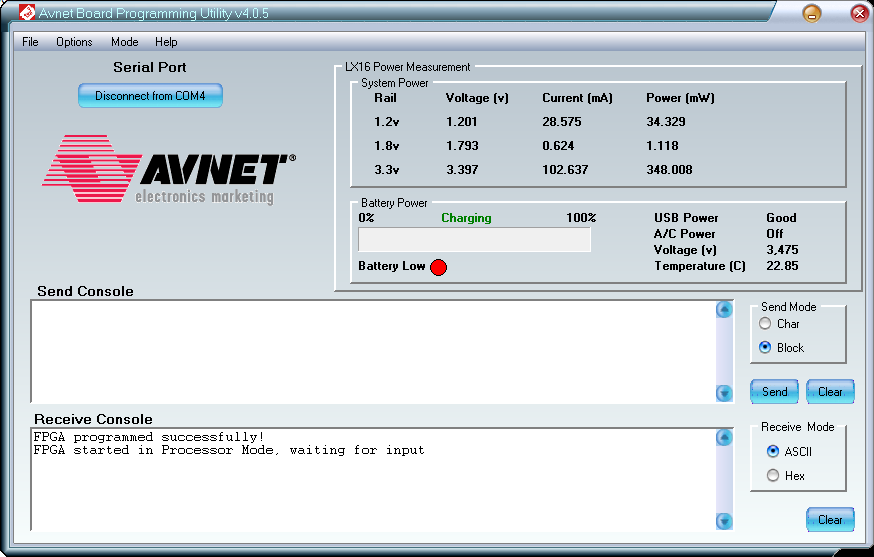
\includegraphics[width=\textwidth]{illustrations/paused.PNG}
\caption{Energy measurements in avProg with the processor not enabled.}
\label{figure-avprog-energy-idle}
\end{figure}

\begin{figure}[H]
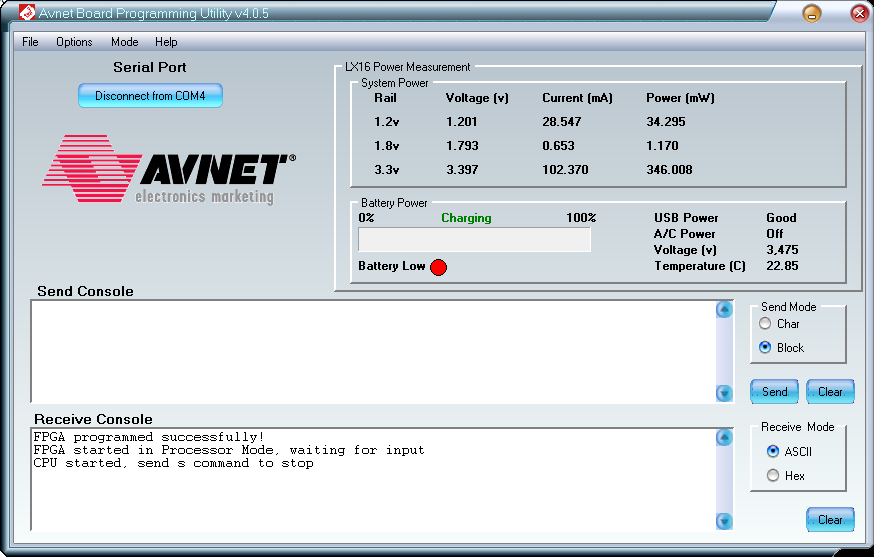
\includegraphics[width=\textwidth]{illustrations/running.PNG}
\caption{Energy measurements in avProg with the processor enabled.}
\label{figure-avprog-energy-running}
\end{figure}

\section{VHDL Test Benches}

Every usefully testable component designed in VHDL has a corresponding test bench.
Informally, every \texttt{*.vhd} file has a \texttt{tb\_*.vhd} file.
Testing every component individually ensures a high quality processor implementation, as it is easy to find, isolate and correct bugs.

The test benches were simulated using ISim. See appendix \todo{add an appendix with tb test results, images} for the test results from the individual test benches. 
The test utilities introduced in \cite{assignment-1} were used to automate testing.

\section{Testing on the Spartan-6 FPGA}

The solution processor was programmed onto an FPGA using avProg.
The processor was successfully programmed and run, but reading the data back from the data memory did not work as expected.
Trying to read data from the data memory of the processor resulted in the communications spinning in an eternal loop.

\section{Testing of the compiler}

The compiler was tested on a small collection of short assembly programs.
The output of the compiler was tested against the hand-compiled versions of the same programs.
